\documentclass[11pt,oneside,final]{memoir}

\usepackage{soul}
\usepackage[cmyk]{xcolor}

\usepackage[pdftex]{graphicx}
\graphicspath{{./src-images/}}
\usepackage{eso-pic}

\usepackage{geometry}
\geometry{
paperwidth=5.125in,
paperheight=8.25in,
nohead,
nofoot,
margin=0pt
}
\setstocksize{8.25in}{5.125in}

\usepackage{fontspec}
\setmainfont[Ligatures = TeX]{Shaker 2 Light}

\newfontfamily\titleFont[Ligatures = TeX]{Shaker 2 Light}
%\newfontfamily\subtitleFont[Ligatures = TeX]{Shaker 2 Regular}
\newfontfamily\subtitleFont[Ligatures = TeX]{Shaker 2 Light}
\newfontfamily\authorFont[
    Ligatures = TeX,
    ItalicFont = Shaker 2 Italic
]{Shaker 2 Regular}

\sodef\soTitle{}{.2em}{.5em plus.1em}{.1em plus.1em minus.1em}
\sodef\soSubTitle{}{.07em}{.4em plus.1em}{.1em plus.1em minus.1em}

\pagestyle{empty}

\setlength{\parindent}{0pt}

\begin{document}
\centering
%\pagecolor[cmyk]{0.45,0.45,0.47,0.06}
\pagecolor[RGB]{137, 101, 82}

\AddToShipoutPictureFG*{\put(\LenToUnit{0mm},\LenToUnit{60mm})%
{\begin{minipage}[b]{\paperwidth}\centering%
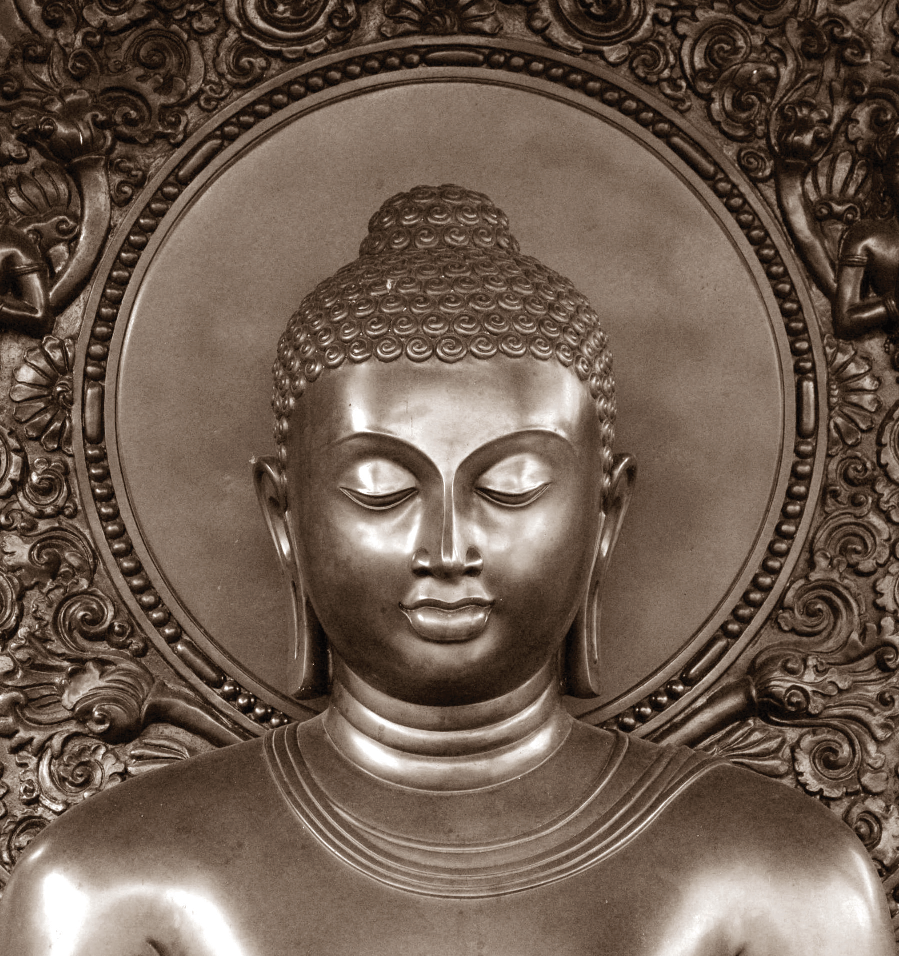
\includegraphics[width=86mm,keepaspectratio]{buddha_sepia.pdf}%
\end{minipage}%
}}%

\vspace*{40mm}

\color[gray]{1}

\resizebox{86mm}{!}{{\titleFont\Huge\MakeUppercase{\soTitle{Dhammapada}}}}

\vspace*{103mm}

{\subtitleFont\Huge \soSubTitle{Az Erény Útja}}
\vspace*{8mm}

{\authorFont\LARGE \textit{Fordította}\\[3mm]\Huge Fórizs László}

\end{document}
